\section{The History}

%	\begin{center} 
%		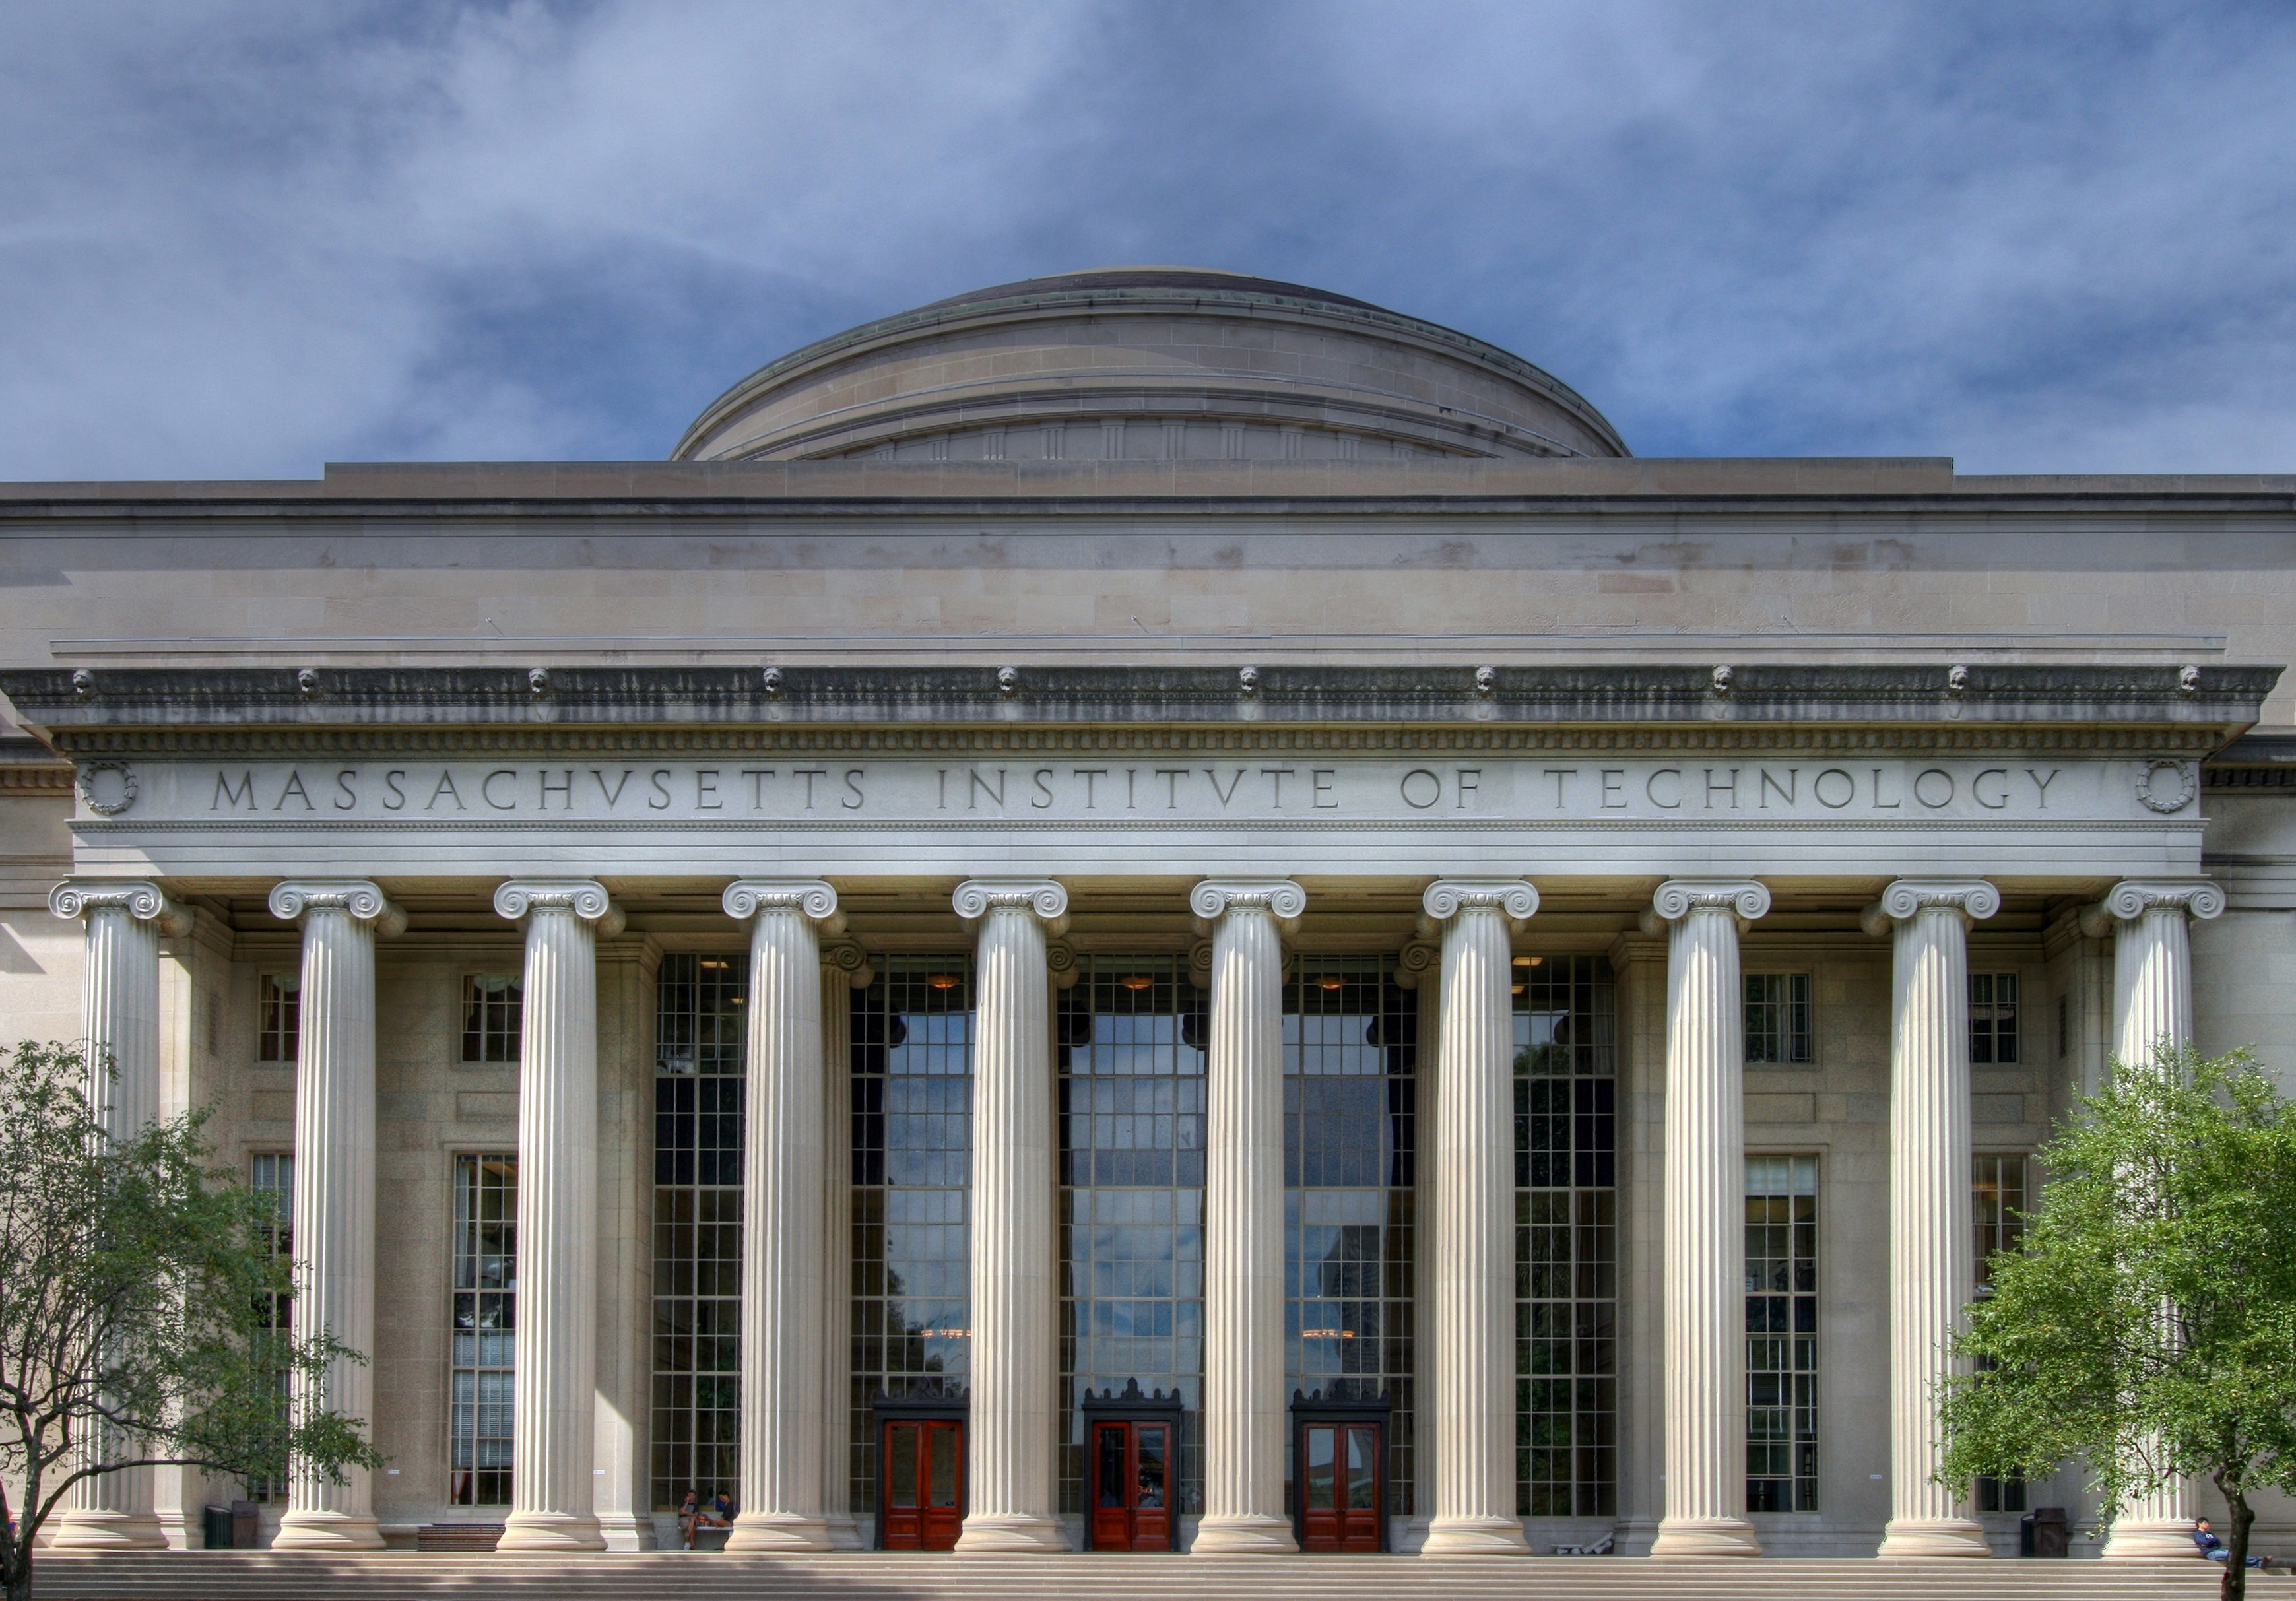
\includegraphics[width=15cm]{img/MIT_Building_10.jpg}
%	\end{center}

\begin{figure}[h]
\center{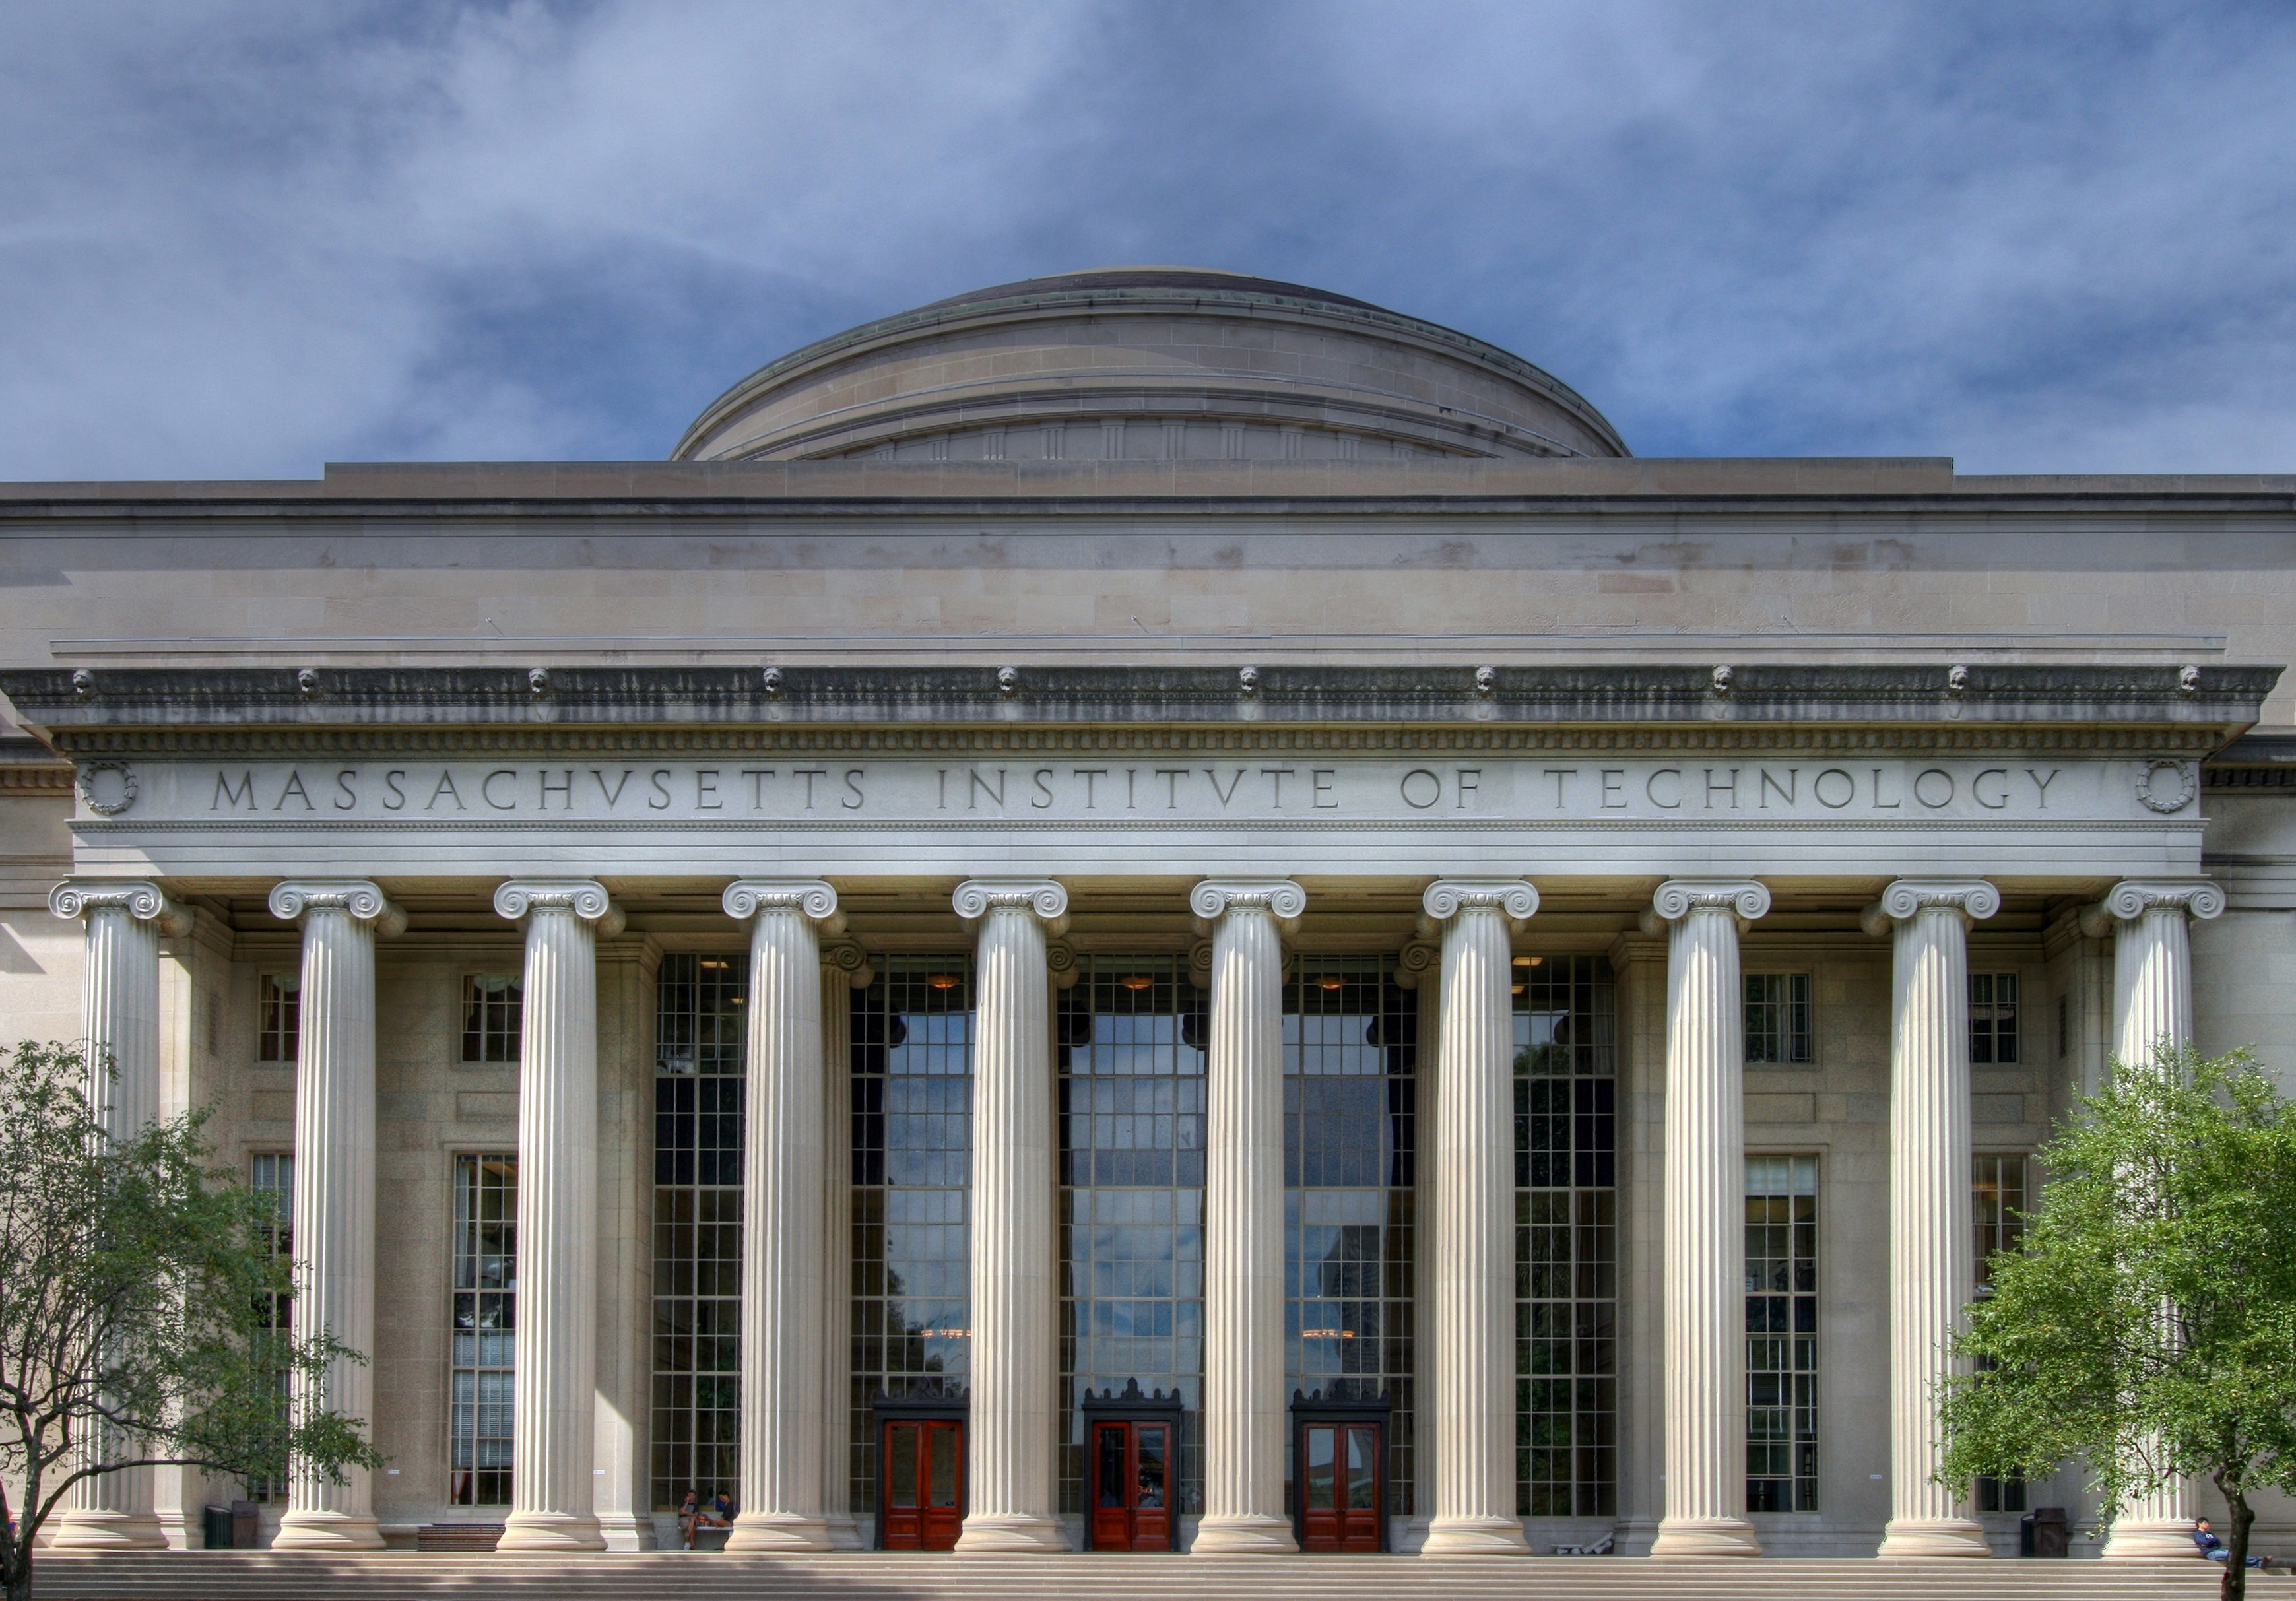
\includegraphics[width=1\linewidth]{img/MIT_Building_10.jpg}}
\caption{MIT's Building 10 and Great Dome overlooking Killian Court}
\end{figure}

The history of the Massachusetts Institute of Technology can be traced back to the 1861 incorporation of the "Massachusetts Institute of Technology and Boston Society of Natural History" led primarily by William Barton Rogers.

\subsection{Vision and mission}

On April 10, 1861, the governor of the Commonwealth of Massachusetts signed a charter for the incorporation of the "Massachusetts Institute of Technology and Boston Society of Natural History" which had been submitted by William Barton Rogers, a natural scientist. Rogers sought to establish a new form of higher education to address the challenges posed by rapid advances in science and technology in the mid-19th century, that he believed classic institutions were ill-prepared to deal with.

\begin{figure}[h]
\center{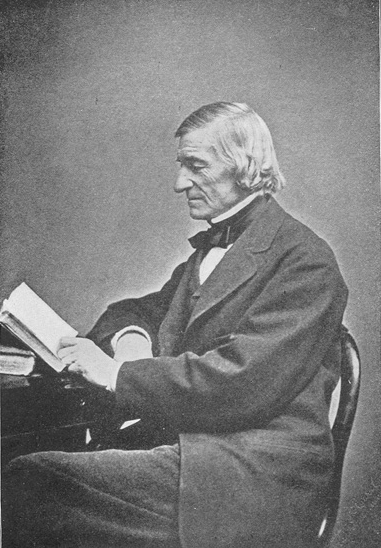
\includegraphics[width=5cm]{img/William_Rogers.jpg}}
\caption{William Barton Rogers}
\end{figure}


With the charter approved, Rogers began raising funds, developing a curriculum and looking for a suitable location. The Rogers Plan, as it came to be known, was rooted in three principles: the educational value of useful knowledge, the necessity of “learning by doing,” and integrating a professional and liberal arts education at the undergraduate level. MIT was a pioneer in the use of laboratory instruction. Its founding philosophy is "the teaching, not of the manipulations and minute details of the arts, which can be done only in the workshop, but the inculcation of all the scientific principles which form the basis and explanation of them;"

Because open conflict in the Civil War broke out only two days later on April 12, 1861, Rogers faced enormous difficulties raising funds to match conditional financial commitments from the state. Thus, his recruitment of faculty and students was delayed, but eventually MIT's first classes were held in rented space at the Mercantile Building in downtown Boston in 1865.

\subsection{Boston Tech (1865–1916)}

Construction of the first MIT building was completed in Boston's Back Bay in 1866 and would be known as "Boston Tech" until the campus moved across the Charles River to Cambridge in 1916.

At the Philadelphia Centennial Exhibition of 1875, Runkle was impressed by the work of the Russian Victor Della-Vos, who had introduced a pedagogical approach combining manual and theoretical instruction at the Moscow Imperial Technical Academy. Runkle became an advocate of this approach, introducing it at MIT.

Francis Amasa Walker was elected President by the MIT Corporation on May 25, 1881. Walker established a new general course of study emphasizing economics, history, law, English, and modern languages. Walker also set out to reform and expand the Institute's organization by creating an Executive Committee, apart from the fifty-member Corporation, to handle regular administrative issues and emphasized the importance of faculty governance by regularly attending their meetings and seeking their advice on major decisions.

\begin{figure}[h]
\center{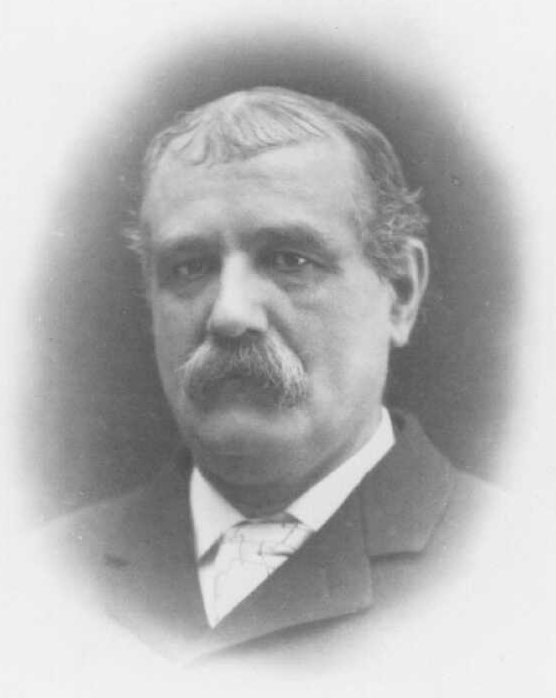
\includegraphics[width=5cm]{img/Francis_Amasa_Walker.jpg}}
\caption{Francis Amasa Walker}
\end{figure}

New programs were also launched under Walker's tenure: Electrical Engineering in 1882, Chemical Engineering in 1888, Sanitary Engineering in 1889, Geology in 1890, Naval Architecture in 1893.

MIT was the first university in the nation to have a curriculum in: architecture (1865), electrical engineering (1882), sanitary engineering (1889), naval architecture and marine engineering (1895), aeronautical engineering (1914), meteorology (1928), nuclear physics (1935), and artificial intelligence (1960s).

\subsection{World War I (1917–1939)}

A pilot training program was necessary as the United States Navy prepared for the emerging technology of naval aviation for World War I. Following the United States declaration of war on 6 April 1917, the Navy implemented a three-part pilot training program beginning with two months of ground school, followed by preliminary flight training teaching student pilots to fly solo, and advanced flight training to qualification as a naval aviator with a commission in the Naval Reserve Flying Corps.

Commander Jerome Clarke Hunsaker, who had previously studied and then taught at the MIT School of Aeronautical Engineering, encouraged the Secretary of the Navy to establish the Navy's first ground school for pilot training at MIT. The first class of fifty student pilots arrived on 23 July 1917 for an eight-week training program covering electricity, signals, photography, seamanship, navigation, gunnery, aeronautic engines, theory of flight, and aircraft instruments.


\subsection{World War II and Cold War (1940–1966)}

MIT was drastically changed by its involvement in military research during World War Two. Bush, who had been MIT's Vice President (effectively Provost) was appointed head of the Office of Scientific Research and Development which was responsible for the Manhattan Project. Government-sponsored research had contributed to a fantastic growth in the size of the Institute's research staff and physical plant as well as a shifting the educational focus away from undergraduates to graduate studies.

As the Cold War and Space Race intensified and concerns about the technology gap between the U.S. and the Soviet Union grew more pervasive throughout the 1950s and 1960s, MIT's involvement in the military-industrial complex was a source of pride on campus.

\subsection {Social movements and activism (1966–1980)}

\subsubsection {Co-education}

\begin{figure}[h]
\center{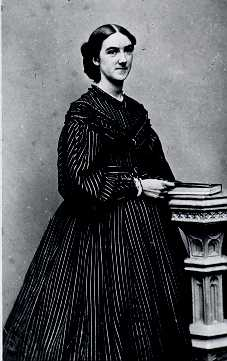
\includegraphics[width=5cm]{img/Ellen_Swallow_Richards.jpg}}
\caption{Ellen Swallow Richards}
\end{figure}

MIT has been nominally coeducational since admitting Ellen Swallow Richards in 1870. Female students, however, remained a tiny minority (numbered in dozens) prior to the completion of the first women's dormitory, McCormick Hall, in 1964. Women constituted 45\% of the undergraduates and 31\% of the graduate students enrolled in 2013. Richards also became the first female member of MIT's faculty, specializing in environmental health.

\subsubsection{Anti-war protests}

However, by the late 1960s and early 1970s, intense protests by student and faculty activists against military-related research required that the MIT administration spin these laboratories off into what would become the Charles Stark Draper Laboratory and Lincoln Laboratory. The extent of these protests is reflected by the fact that MIT had more names on "President Nixon's enemies list" than any other single organization, among them its president Jerome Wiesner and professor Noam Chomsky. Memos revealed during Watergate indicated that Nixon had ordered MIT's federal subsidy cut "in view of Wiesner's anti-defense bias."

\subsubsection {Social movements}

MIT's particular strain of anti-authoritarianism has manifested itself in other forms. In 1977, two female students, juniors Susan Gilbert and Roxanne Ritchie, were disciplined for publishing an article on April 28 of that year in the "alternative" MIT campus weekly Thursday. Entitled "Consumer Guide to MIT Men," the article was a sex survey of 36 men the two claimed to have had sex with, and the men were rated according to their performance. Gilbert and Ritchie had intended to turn the tables on the rating systems and facebooks men use for women, but their article led not only to disciplinary action against them but also to a protest petition signed by 200 students, as well as condemnation by President Jerome B. Wiesner, who published a fierce criticism of the article.


